\documentclass[12pt, a4paper, oneside]{ctexbook}
\usepackage{amsmath, amsthm, amssymb, bm, graphicx, hyperref, mathrsfs}
\usepackage{geometry}
\usepackage{subfigure}
\usepackage{hyperref}[colorlinks=true,linkcolor=blue,citecolor=blue,urlcolor=blue,]
\usepackage{pdfpages}
\usepackage{svg}
\usepackage{url}

\usepackage{multirow}
\usepackage{xcolor}[table,xcdraw]

%设置引用格式
\hypersetup{
	colorlinks=true,linkcolor=black,colorlinks=true,linkcolor=black,citecolor=blue,urlcolor=blue
}
%在LateX中,参考文献的引用一般有两种方式,平 齐 时 用 命 令\cite{...}, 上 标 时用\textsuperscript{\cite{...}}

\CTEXsetup[format={\Large\bfseries}]{section}	%section 居左(默认居中)
\CTEXsetup[format={\huge\bfseries}]{chapter}	%chapter 居左(默认居中)


%配置纸张边缘
\geometry{left=2.54cm,right=2.54cm,top=3.18cm,bottom=3.18cm}


\title{{\Huge{\textbf{仿真验证环境说明文档}}}\normalsize{\\——第六届全国大学生集成电路创新创业大赛景嘉微杯分赛区决赛提交文档}}
\author{队名:虹ヶ咲学园芯片设计同好会\\ 成员:黄金源\space邓立唯\space林明锋}
\date{\today}
\linespread{1.5}


\begin{document}
	%-----------------------封面------------------
	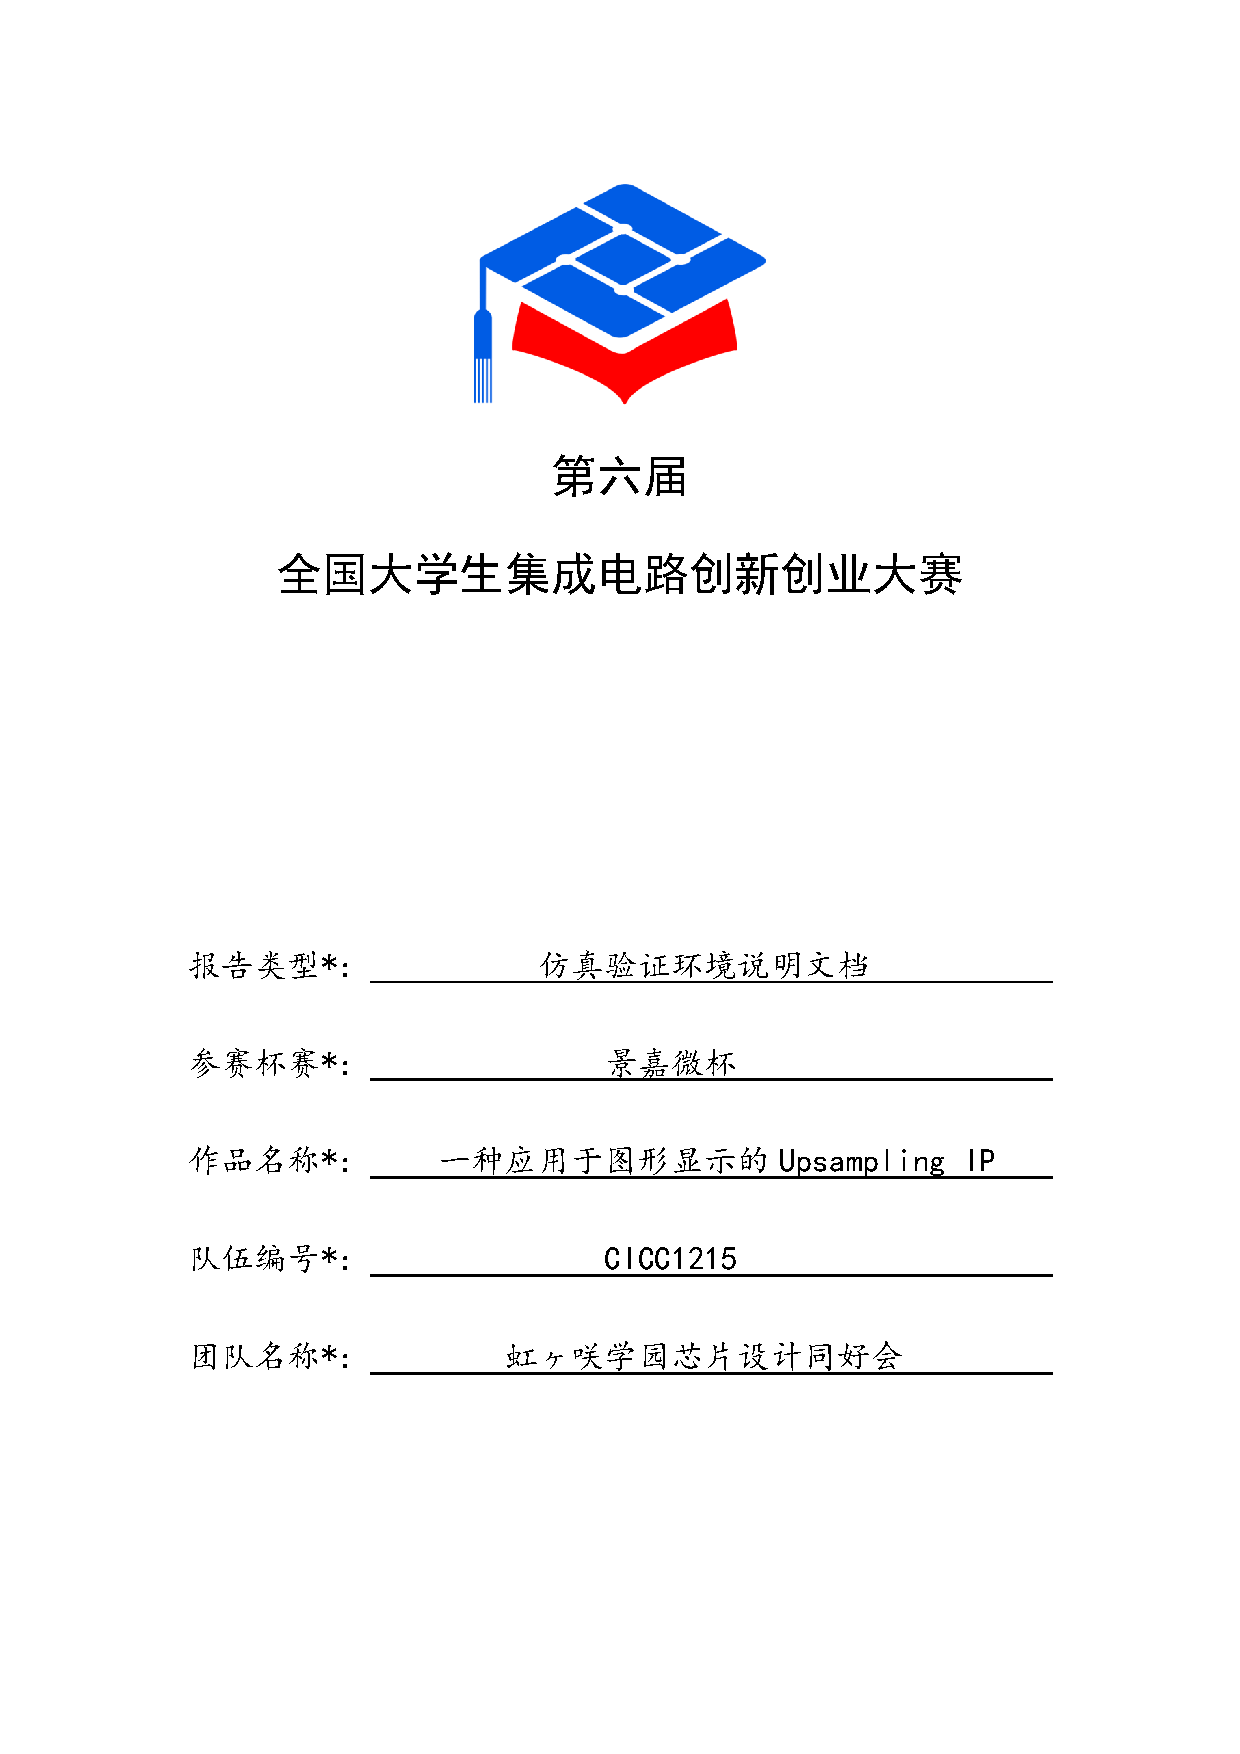
\includepdf{./pic/cover.pdf}
	\maketitle	
	\pagenumbering{Roman}
	\setcounter{page}{1}
	%-----------------------前言------------------
	\begin{center}
		\Huge\textbf{前言}
	\end{center}~\
	
	本文档(仿真验证环境及说明文档)仅作为虹ヶ咲学园芯片设计同好会(成员:黄金源、邓立唯、林明锋)参加第六届全国大学生集成电路创新创业大赛景嘉微杯赛分赛区决赛提交文档供评委评分使用。
	~\\
	\begin{flushright}
		\includegraphics[width=0.25\linewidth]{pic/logo}\\
		\begin{tabular}{c}
			虹ヶ咲学园芯片设计同好会\\
			\today
		\end{tabular}
	\end{flushright}
	%-----------------------目录------------------
	\newpage
	\pagenumbering{Roman}	%Roman or arabic
	\setcounter{page}{1}
	\tableofcontents
	\newpage
	\setcounter{page}{1}
	\pagenumbering{arabic}
	
	%-----------------------正文----------------	
	\chapter{验证工具}
	本次 IP 验证平台将基于 System Verilog 进行编写。\par 使用由队伍成员邓立唯开源的 \href{https://github.com/Aperture-Electronic/SystemVerilog-Bitmap-Library-AXI-Image-VIP}{\textit{Bitmap Processing Library \& AXI-Stream Video Image VIP}} 进行测试样例图片读取写回,简化测试样例生成步骤及测试结果输出对比。\par \par
	\emph{To verificate a video or a image processing IP, you may need to read a real image into your design, send its data by an interface. Then, get the output from the interface, and convert it to a new image, save or compare it. ——\href{https://github.com/Aperture-Electronic/SystemVerilog-Bitmap-Library-AXI-Image-VIP}{Bitmap Processing Library \& AXI-Stream Video Image VIP}} \\
	
	\par \par 由于队伍成员每个人有不同的验证工具使用习惯,在本次项目验证中将会使用到:
	\begin{itemize}
		\item Intel ModelSim
		\item Synopsys VCS \& Verdi
		\item Verilator \& GtkWave
	\end{itemize}
	\chapter{验证方法及策略}
	采用 \textbf{直接验证} 与 \textbf{随机验证} 结合。\\ \\
	\textbf{直接验证}: 通过对比测试图片在 C Model 进行超分辨率算法运算结果与 RTL 代码在仿真中输出结果对比。\\
	\textbf{随机验证}: 对部分子模块(如高斯滤波器、纹理分类器等)所需的运算数据通过产生随机种子产生随机数据,对比参考模型运算输出结果与待测模块输出结果。
	
	
	\chapter{验证范围}
		\section{各子运算单元}
		\begin{itemize}
			\item 运算结果正确
			\item 运算结果有效输出
			\item 结果输出是否超出数据范围
			\item 满足时序要求
		\end{itemize}
	
		\section{Bicubic 上采样模块}
		\begin{itemize}
			\item 满足 AXI4-Stream 协议要求,完成视频流数据收发
			\item 完成 Biubic 上采样算法结果输出
			\item 运算结果与参考模型匹配
			\item 结果输出是否超出数据范围
			\item 支持视频帧停顿
			\item 满足时序要求
		\end{itemize}
	
		\section{纹理分类模块}
		\begin{itemize}
			\item 满足 AXI4-Stream 协议要求,完成视频流数据接收
			\item 完成纹理分类算法结果输出
			\item 输出寻址结果与参考模型匹配
			\item 结果输出是否超出地址范围
			\item 支持视频帧停顿
			\item 满足时序要求
		\end{itemize}

		\section{自适应锐化模块}
		\begin{itemize}
			\item 满足 AXI4-Stream 协议要求,完成视频流数据收发
			\item 完成自适应锐化算法结果输出
			\item 输出像素结果与参考模型匹配
			\item 结果输出是否超出数据范围
			\item 支持视频帧停顿
			\item 满足时序要求		
		\end{itemize}
	
		\section{色域转换模块}
		\begin{itemize}
			\item 满足 AXI4-Stream 协议要求,完成视频流数据收发
			\item 完成色域转换运算结果输出
			\item 输出像素结果与参考公式一致
			\item 结果输出是否超出数据范围
			\item 满足时序要求		
		\end{itemize}
	
		\section{注意事项}
		\begin{itemize}
			\item 不需进行跨时钟域检查
			\item 需进行覆盖率验证	
		\end{itemize}		
		
		
	\chapter{验证环境}
		\section{验证平台}
		该验证平台包含了测试样例生成器、驱动器、待测单元、其他外设VIP(如DDR)、监视器、记分板、参考模型以及一个全局配置。	
		\begin{figure}[h]
			\centering
			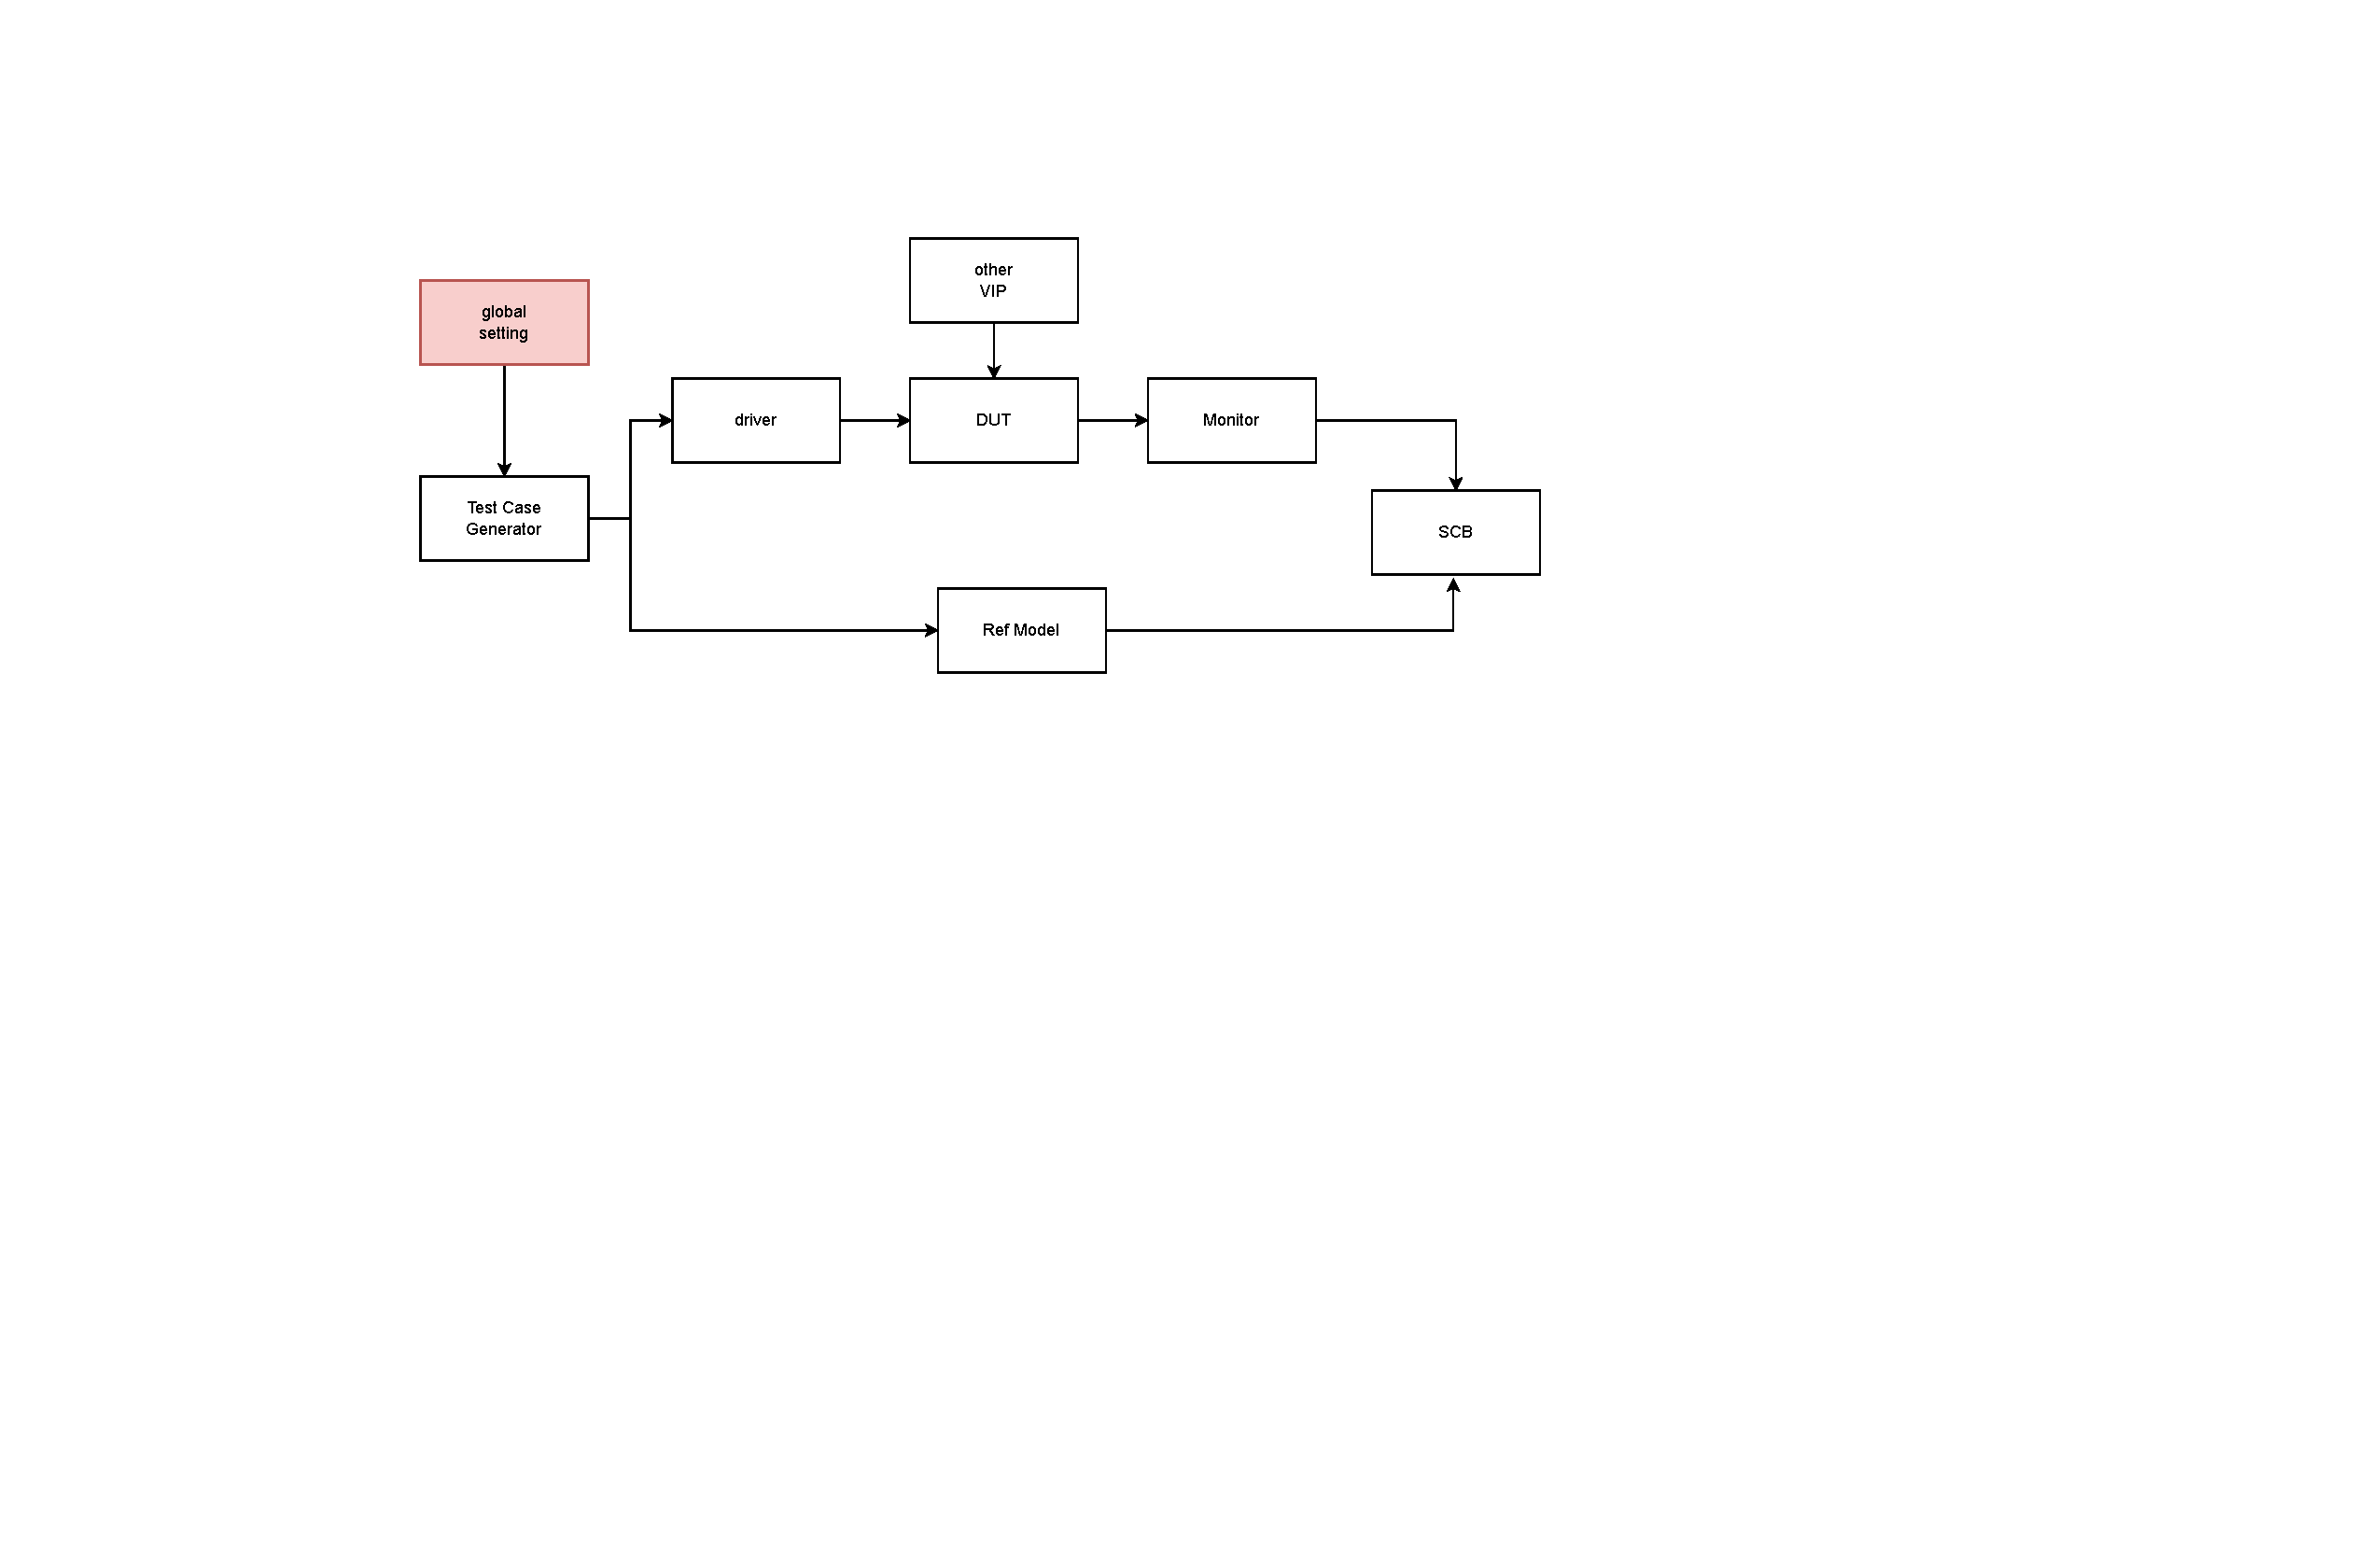
\includegraphics[scale=0.7]{pic/testbench}
			\caption{验证平台}
			\label{fig:testbench}
		\end{figure}

		\section{验证计划}
		\begin{itemize}
			\item 使用 60 组真实图片进行验证;
   			\item 使用 100 组随机生成图片进行验证;
      		\item 使用极端数值进行验证;
        	\item 使用随机数值进行验证。
		\end{itemize}

		\section{待验证设计}
			无待验证设计

		\section{完成验证设计}
			\begin{itemize}
				\item 各子运算单元
				\item Bicubic 上采样模块
				\item 纹理分类模块
				\item 自适应锐化模块
				\item 色域转换模块
			\end{itemize}
	\chapter{覆盖率}
	\section{各子运算单元}
	该单元无收集验证覆盖率。
	\section{Bicubic 上采样模块}
	详细验证覆盖率结果可参考文档 \href{./ref/APV21B_Simulation_Verification_Enviroment.pdf}{\textit{APV21B-Simulation \& Verification Enviroment}}。
	\section{纹理分类模块}
	详细验证覆盖率结果可查看 \href{file:./coverage_report/textureclassifier/dashboard.html}{\textit{纹理分类模块覆盖率报告}}。
	\section{自适应锐化模块}
	详细验证覆盖率结果可查看 \href{file:./coverage_report/adaptedSharpener/dashboard.html}{\textit{自适应锐化模块覆盖率报告}}。
	\section{色域转换模块}
		\subsection{RGB2YUV Unit}
		详细验证覆盖率结果可查看 \href{file:./coverage_report/rgb2yuv/dashboard.html}{\textit{RGB2YUV Unit Coverage Report}}。
		\subsection{YUV2RGB Unit}
		详细验证覆盖率结果可查看 \href{file:./coverage_report/yuv2rgb/dashboard.html}{\textit{YUV2RGB Unit Coverage Report}}。
	
	\chapter{验证分析}
	\section{各子运算单元}
	符合设计预期。
	\section{Bicubic 上采样模块}
	符合设计预期。
	\section{纹理分类模块}
	验证结果设计需要更完备,测试条件未覆盖完全。
	\section{自适应锐化模块}
	验证结果设计需要更完备,测试条件未覆盖完全。
	\section{色域转换模块}
	符合设计预期。


\end{document}
